% Introducción
\begin{frame}
  \frametitle{Introducción}
  \framesubtitle{Problemas de iluminación.} %%Subtítulo de la diapositiva (opcional)
  Un problema de iluminación consta de iluminar áreas específicas con fuentes. Las fuentes de luz
  utilizadas para iluminar nuestros objetos pueden ser de varios tipos, lámparas que emiten luz
  alrededor de ellas, reflectores o fuentes de luz que solo iluminan dentro de una zona angular, etc.

  %\centering \includegraphics[width=0.35 \paperwidth]{images/Iluminación.png}
  \begin{figure}
    \centering
    \includegraphics[width=0.35 \paperwidth]{./images/Iluminación.png}
    \caption*{Iluminación.}
  \end{figure}
  
  %\begin{itemize}
  %  \item[\checkmark] Un elemento en la lista %%[\checkmark] muestra una palomita al inicio de la línea
  %  \item Segundo elemento
  %  \item Otro elemento
  %  \item Y finalmente, otro más
  %\end{itemize}
\end{frame}

\begin{frame}
  \frametitle{Introducción}
  \framesubtitle{Problemas de visualización.} %%Subtítulo de la diapositiva (opcional)
  Intimamente ligado a los problemas de iluminación está el estudio de gráficas
  de visibilidad. Dado un polıígono $P$ en el plano, la gráfica de visibilidad
  interna de $P$ es la gráfica cuyos vértices son los vértices de $P$, en la cual dos
  vértices son adyacentes, si el segmento de línea que los une está totalmente
  contenido en $P$ (análoga la definición externa).

  %\centering \includegraphics[width=0.35 \paperwidth]{images/Iluminación.png}
  \begin{figure}
    \centering
    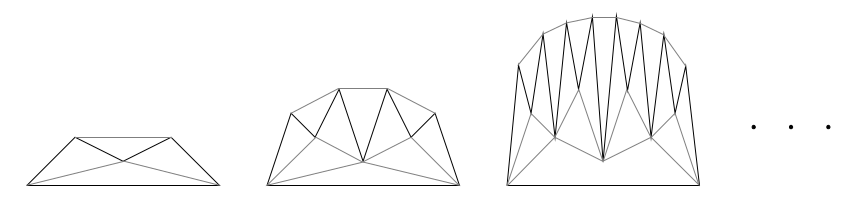
\includegraphics[width=0.55 \paperwidth]{./images/GraphVisibility.png}
    \caption*{Gráficas de visibilidad en una familia de polígonos.}
  \end{figure}
  
  %\begin{itemize}
  %  \item[\checkmark] Un elemento en la lista %%[\checkmark] muestra una palomita al inicio de la línea
  %  \item Segundo elemento
  %  \item Otro elemento
  %  \item Y finalmente, otro más
  %\end{itemize}
\end{frame}
